% !TeX spellcheck = de_CH_frami

\section{MOS-Stromspiegel (Kap. 9)}

\begin{minipage}[t]{0.25\textwidth}
	\textbf{Stromspiegelverhältnis}\\
	$n_m=\frac{I_{out}}{I_{in}}=\frac{(\frac{W}{L})_{2}}{(\frac{W}{L})_{1}}$
\end{minipage}
\begin{minipage}[t]{0.35\textwidth}
	\textbf{Berechnung Ausgangsstrom}\\
	$I_{out}=I_{in}\cdot\frac{(\frac{W}{L})_{2}}{(\frac{W}{L})_{1}}$ (allgemein)\\
	$I_{out}=I_{in}\cdot \frac{W_{T2}}{W_{T1}}$ (wenn $L_{T2}=L_{T1}$)
\end{minipage}
\begin{minipage}[t]{0.35\textwidth}
	\textbf{Impedanzen}\\
	Eingangsimpedanz (ideal): $r_{in}=0\Omega$\\
	Ausgangsimpedanz (ideal): $r_{out}=\infty\Omega$
\end{minipage}\\
\begin{tabular}{|p{0.4\textwidth}|p{0.525\textwidth}|}
	\hline
	\textbf{Widlar-Stromspiegel}&\textbf{Wilson-Stromspiegel}\\
	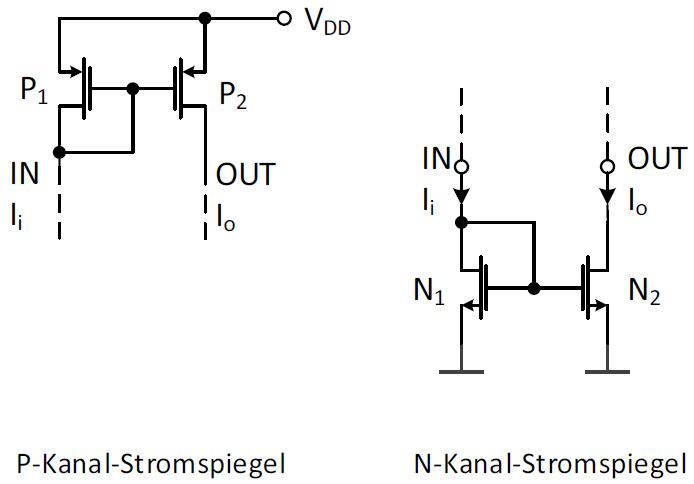
\includegraphics[height=5cm]{chapters/Stromspiegel/images/Widlar}&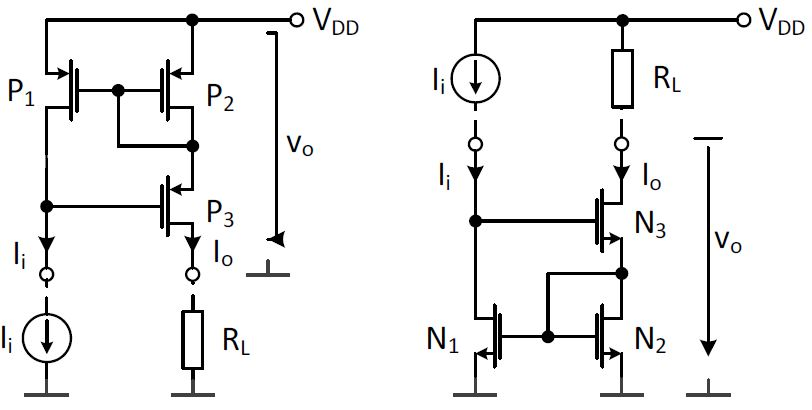
\includegraphics[height=5cm]{chapters/Stromspiegel/images/Wilson}\\ \hline
\end{tabular}\\
\begin{tabular}{|p{0.25\textwidth}|p{0.25\textwidth}|p{0.402\textwidth}|}
	\hline
	\textbf{verbesserter Wilson-Stromspiegel}&\textbf{Kaskode}&\textbf{geregelte Kaskode}\\
	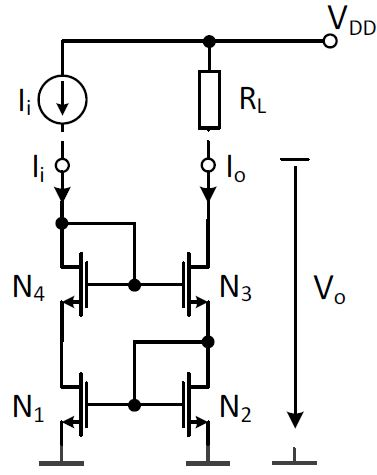
\includegraphics[height=5cm]{chapters/Stromspiegel/images/verbesserterWilson}&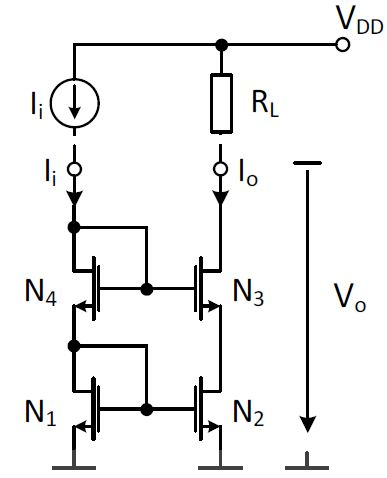
\includegraphics[height=5cm]{chapters/Stromspiegel/images/Kaskode}&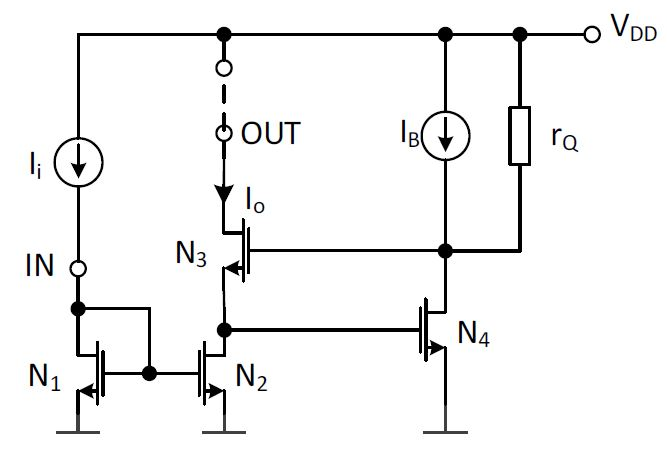
\includegraphics[height=5cm]{chapters/Stromspiegel/images/geregelteKaskode}\\ \hline
\end{tabular}\\[2ex]
\begin{tabular}{|l|l|l|l|l|}
	\hline
	\textbf{Stromspiegeltyp}&\textbf{Genauigkeit}&\textbf{$r_{out}$}&\textbf{$V_I$}&\textbf{$V_{O,min}$}\\ \hline
	Widlar-Stromspiegel&+&$=\frac{1}{g_0}$&$\approx V_T + \sqrt{\frac{2I_I}{\beta}}$&$\approx \sqrt{\frac{2I_0}{\beta}}$\\ \hline
	Wilson-Stromspiegel&+&$\approx \frac{1}{g_0}(2+\frac{g_m}{g_0})$&$\approx 2V_T+2\sqrt{\frac{2I_I}{\beta}}$&$\approx V_T+2\sqrt{\frac{2I_0}{\beta}}$\\ \hline
	Verbesserter Wilson&++&$\approx \frac{1}{g_0}(2+\frac{g_m}{g_0})$&$\approx 2V_T+2\sqrt{\frac{2I_I}{\beta}}$&$\approx V_T+2\sqrt{\frac{2I_0}{\beta}}$\\ \hline
	Kaskode-Stromspiegel&++&$\approx \frac{1}{g_0}(2+\frac{g_m}{g_0})$&$\approx 2V_T+2\sqrt{\frac{2I_I}{\beta}}$&$\approx V_T+2\sqrt{\frac{2I_0}{\beta}}$\\ \hline
	geregelte Kaskode&++&$\approx\frac{1}{g_0}(\frac{g_m}{g_0})^2$&$\approx V_T+\sqrt{\frac{2I_I}{\beta}}$&$\approx 2\sqrt{\frac{2I_0}{\beta}}$\\ \hline
\end{tabular} \\ [1ex]
\textbf{Beeinflussung von Stromspiegelverhältnis mittels hinzufügen von Sourcewiderstand} \\
